\subsection{Radiant}\label{2-fundamentacao-ferramentas-radiant}

Radiant~\cite{MILLER-VERMA-GOMADAM-SHETH-BREWER-2005-Radiant} é um \textit{plugin} do IDE Eclipse. Radiant faz parte do conjunto de ferramentas METEOR-S, usadas para criação de processos e serviços web semânticos. Radiant provê suporte para as linguagens \textit{Web Service Semantics} (WSDL-S)~\cite{W3C-2005-WSDL-S} e SAWSDL~\cite{W3C-2007-SAWSDL}, permitindo que usuários adicionem, por meio de uma interface gráfica, anotações semânticas às descrições de serviços web~\cite{MILLER-VERMA-GOMADAM-SHETH-BREWER-2005-Radiant}. Para facilitar a compreensão dos conceitos de uma ontologia envolvidos na anotação semântica, Radiant também provê um visualizador de ontologia.

Radiant abstrai parcialmente detalhes técnicos de documentos WSDL e OWL, facilitando a tarefa de anotar um serviço web. A abstração ocorre por meio da representação visual de elementos de uma descrição de serviço web (WSDL) e de uma ontologia em um formato de árvore (\textit{tree-view}). A \figurename~\ref{fig:radiant} ilustra a interface gráfica de Radiant. Na lateral esquerda, encontram-se representados os elementos WSDL. Na lateral direita, encontram-se representados os elementos de uma ontologia. Finalmente, no centro, encontra-se a especificação WSDL anotada.

Por meio de Radiant, também é possível anotar um documento WSDL utilizando o recurso \textit{drag-and-drop}. O usuário pode arrastar um conceito de uma ontologia para cima de um elemento WSDL. Com isso, a anotação semântica é adicionada automaticamente ao documento WSDL. As anotações semânticas podem ser vistas na visualização do código WSDL/XML, por meio do painel central.

Apesar destas representações visuais (abstrações parciais) contribuírem para uma melhor compreensão dos elementos envolvidos na anotação semântica, ainda faz-se necessário lidar diretamente com código WSDL/XML de descrições de serviços e de atributos SAWSDL. Adicionalmente, o usuário necessita percorrer uma ontologia inteira a fim de obter os conceitos apropriados para a anotação semântica de um serviço web. Como uma ontologia pode conter um grande conjunto de conceitos e relacionamentos, anotar semanticamente um serviço pode requerer um esforço significativo.

\begin{figure}[h]
    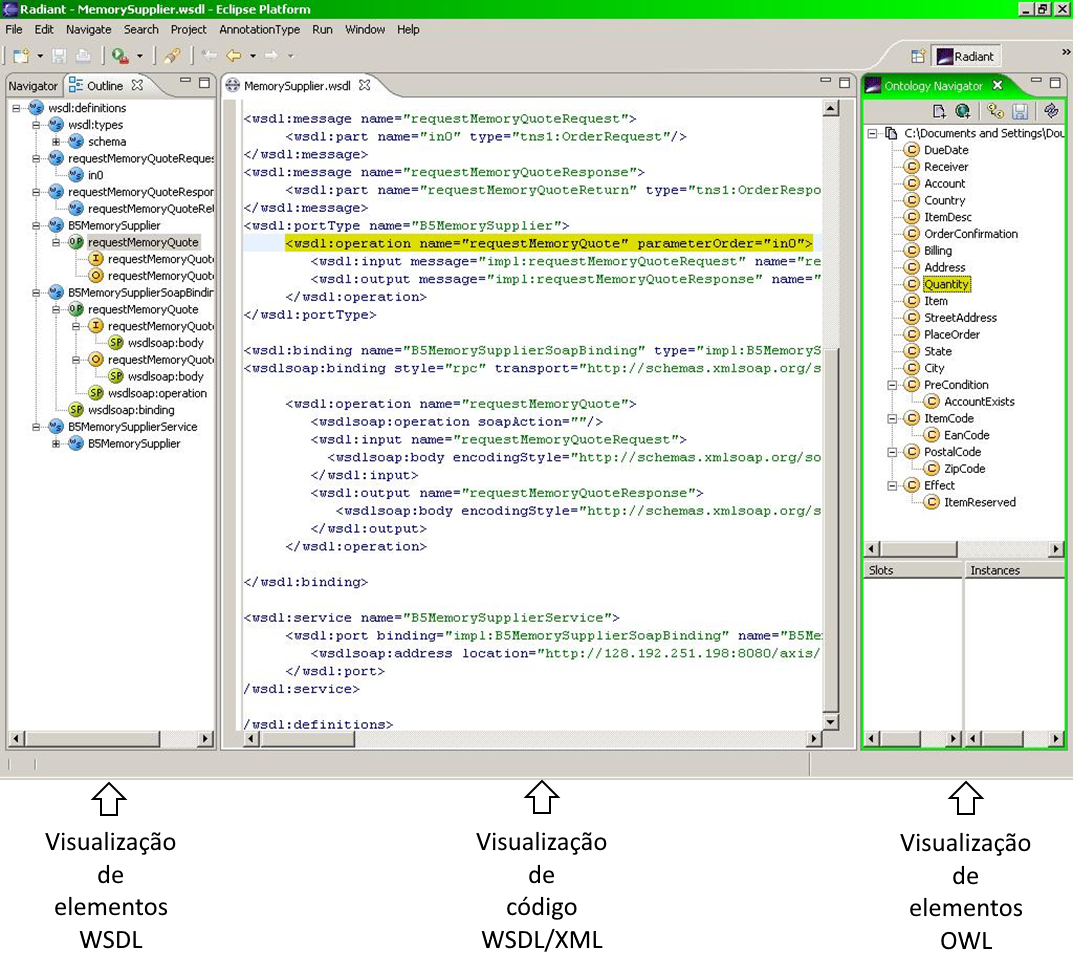
\includegraphics[scale=0.5]{2-fundamentacao-teorica/imagens/radiant3.png}
    \centering
    \caption[Interface gráfica de usuário da ferramenta Radiant.]{\textbf{Interface gráfica de usuário da ferramenta Radiant.}}
    \label{fig:radiant}
\end{figure}